\chapter{Entfaltung als Klassifikationsproblem}
\begin{table}
    \centering
    \begin{tabular}{l l l l}
        \toprule
        Ebene & Aktivierungsfunktion & Eingangsdimension & Ausgangsdimension \\
        \midrule
        Eingang & - & $12$ & $12$ \\
        Tief & ReLU & $12$ & $120$ \\
        Tief & ReLU & $120$ & $240$ \\
        Tief & ReLU & $240$ & $120$ \\
        Tief & ReLU & $120$ & $12$ \\
        Ausgang & Softmax & $12$ & $10$ \\
        \bottomrule
    \end{tabular}
    \caption{Die Struktur des neuronalen Netzes von oben nach unten gelesen.
    Die Aktivierungsfunktion und Eingangs- und Ausgangsdimensionen sind für jede Ebene aufgeführt.
    }
    \label{tab:nn_shape}
\end{table}

\begin{table}
    \centering
    \begin{tabular}{l l}
        \toprule
        Parameter & Wert \\
        \midrule
        Epochenzahl & $50$ \\
        Batchgröße & $2048$ \\
        Lernrate (ADAM) & $0.0005$ \\
        \bottomrule
    \end{tabular}
    \caption{Hyperparameter des neuronalen Netzes.}
    \label{tab:nn_params}
\end{table}

\begin{figure}%
    \centering%
    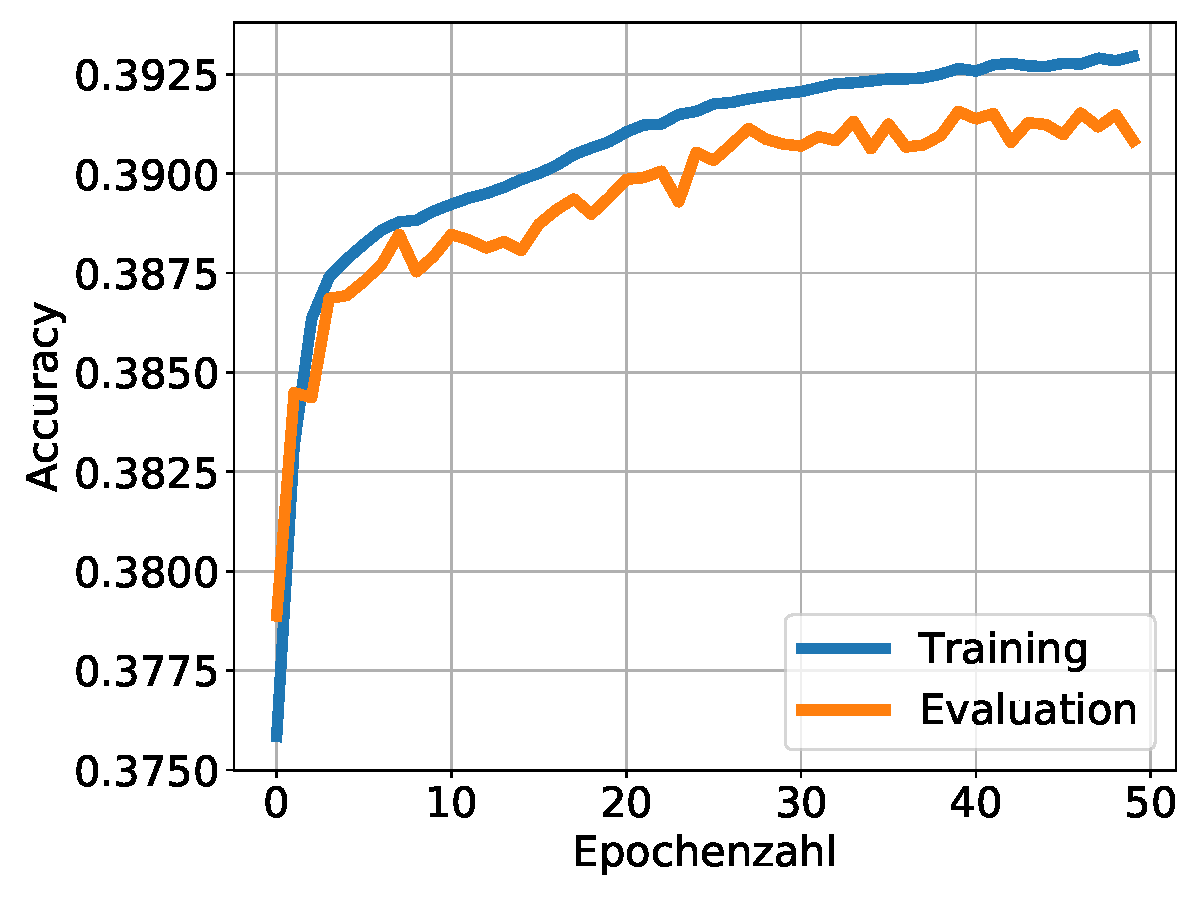
\includegraphics[width=0.7\textwidth]{Plots/NN/acc.pdf}%
    \caption[Verlauf der Accuracy für den Trainingsprozess des NN ohne DSEA]{Verlauf der Accuracy in Abhängigkeit der Epochenzahl für den Trainingsprozess des NN.}%
    \label{fig:NN_acc}%
\end{figure}%

\begin{figure}%
    \centering%
    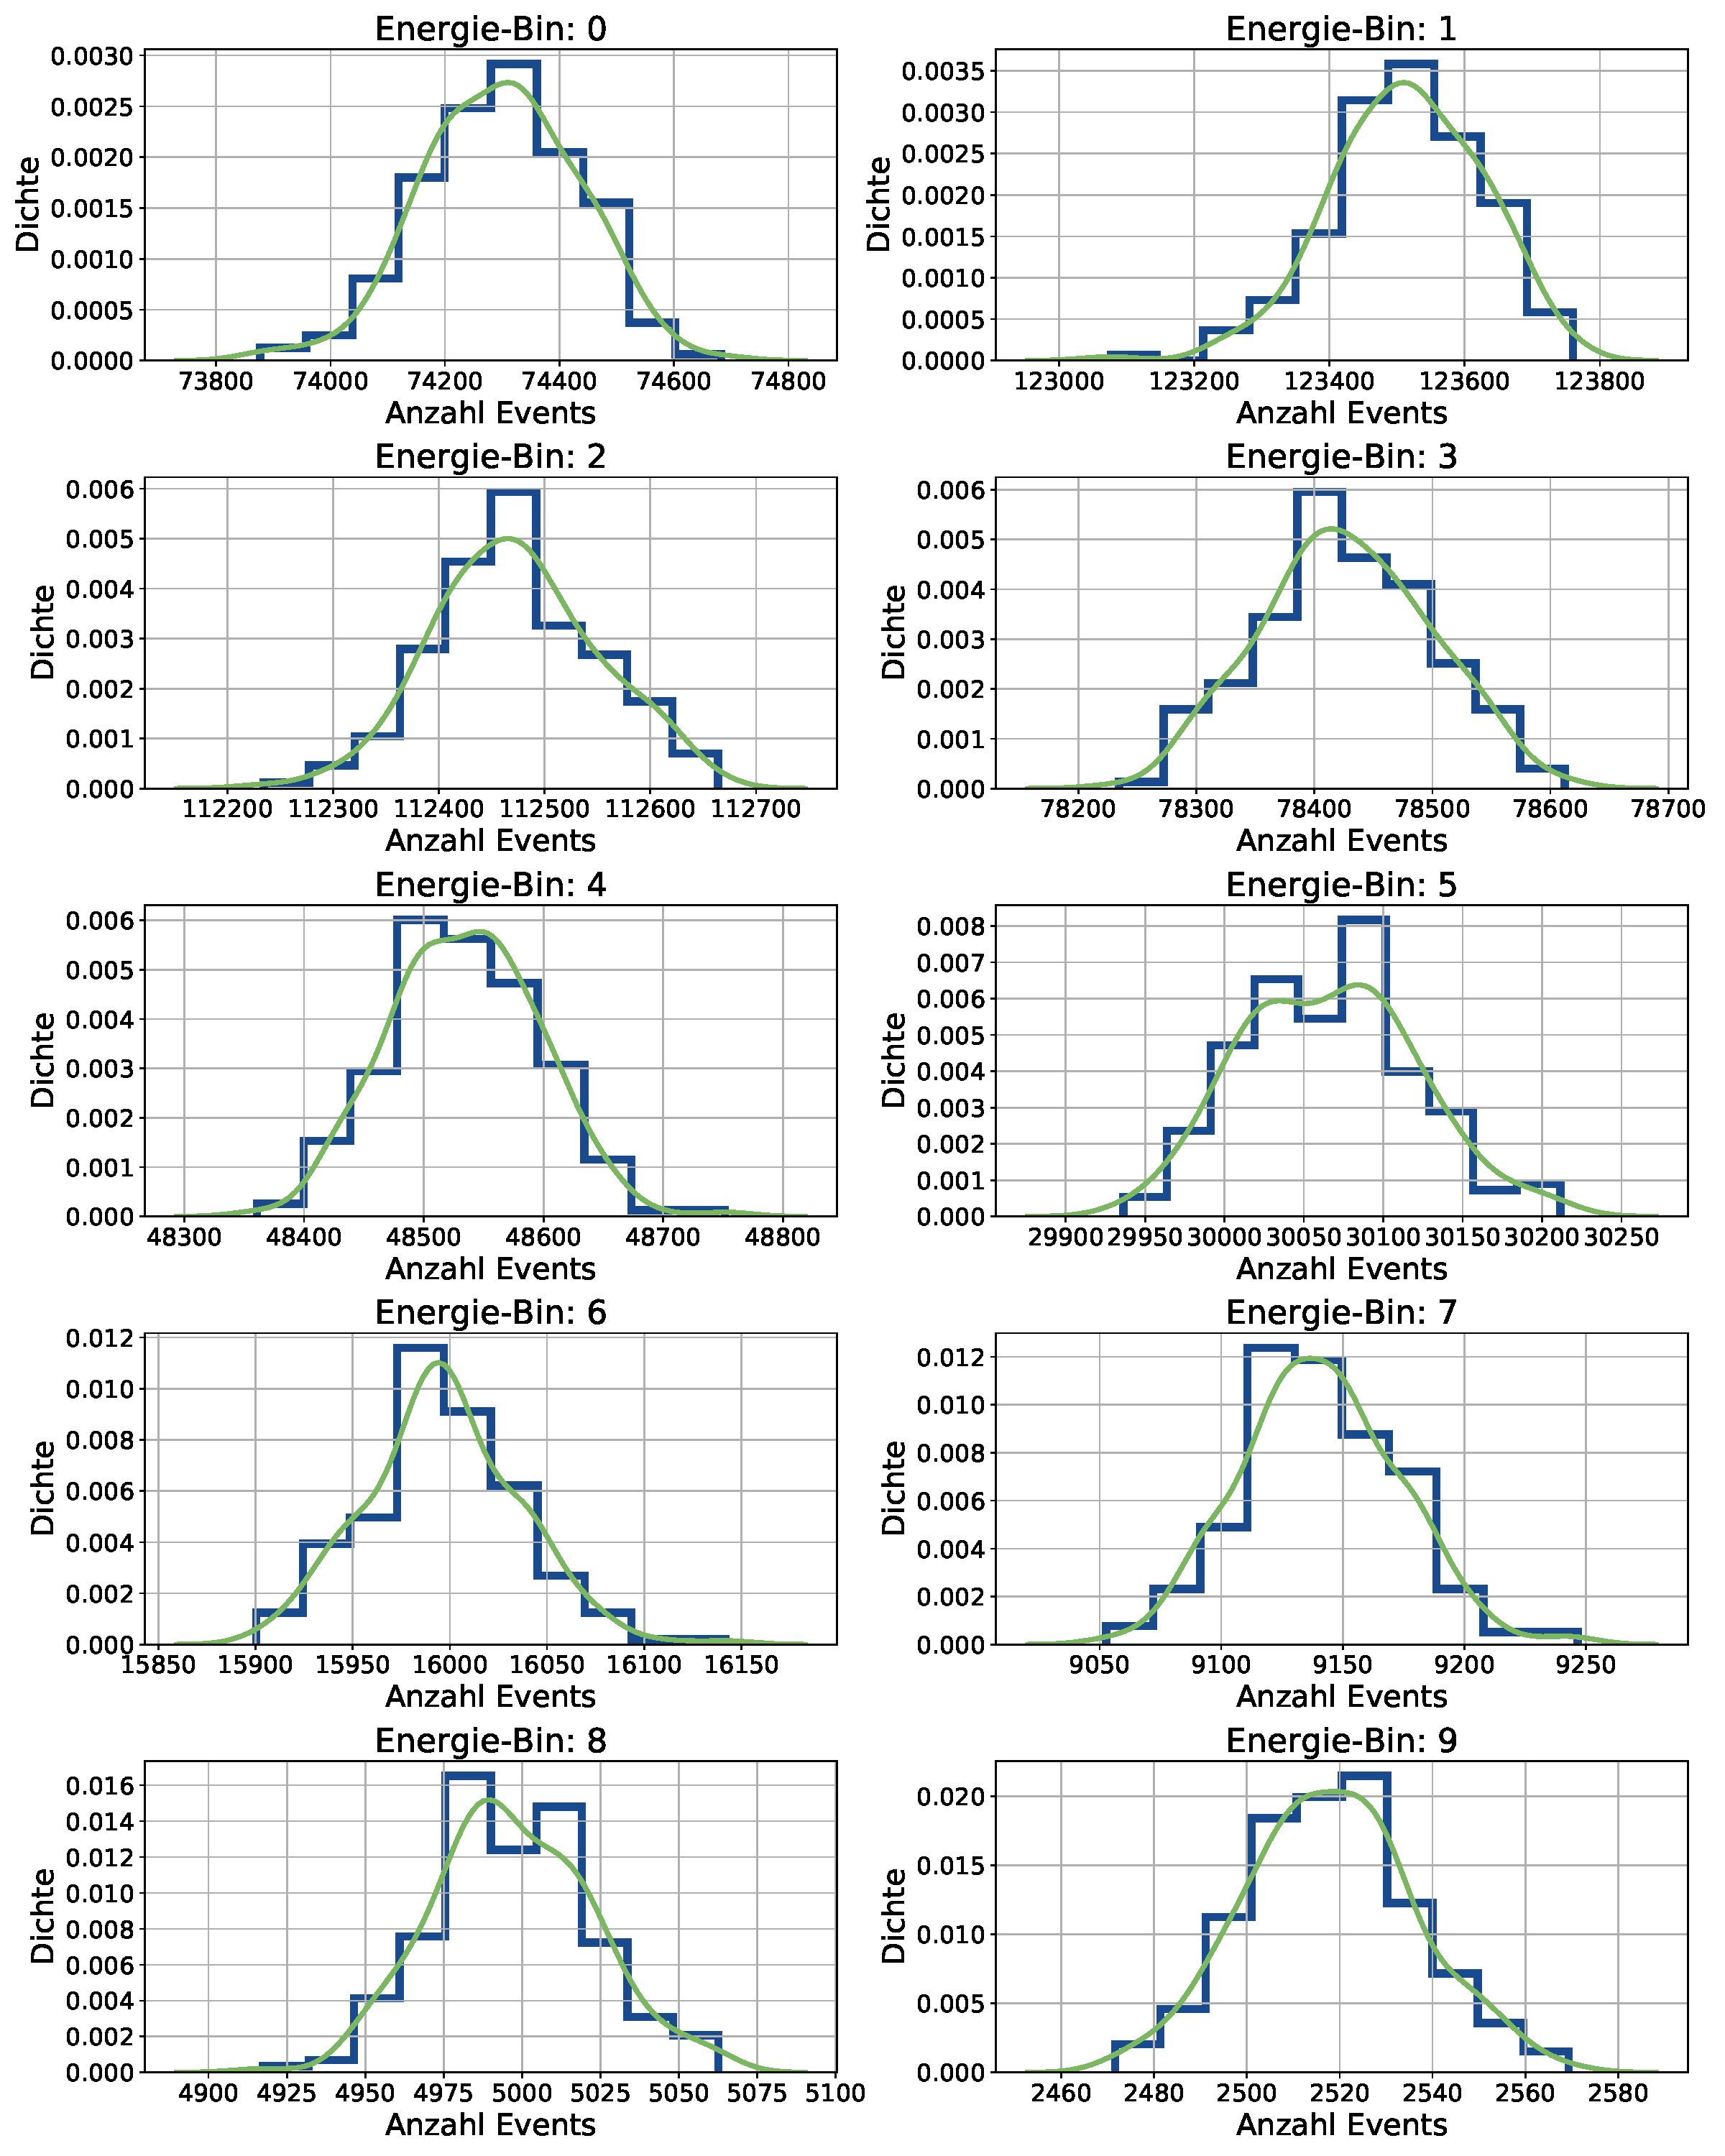
\includegraphics[width=\textwidth]{Plots/NN/class_dist_10bins_50ep_500000samples_200pulls.pdf}%
    \caption[Ergebnisse des Bootstrapping-Vefahrens für das NN ohne DSEA]{Das blaue Histrogramm stellt die Verteilung der Bootstrap-Ergebnisse mit 200 Iterationen dar.
    Die rote Funktion repräsentiert einen Kerndichteschätzer(KDE) mit Gaußkern.
    Die Bin-Höhe wird durch den Median angegeben.
    Über das untere und obere Quantil werden die Unsicherheiten bestimmt.
    }%
    \label{fig:NN_bootstrap}%
\end{figure}%

\begin{figure}%
    \centering%
    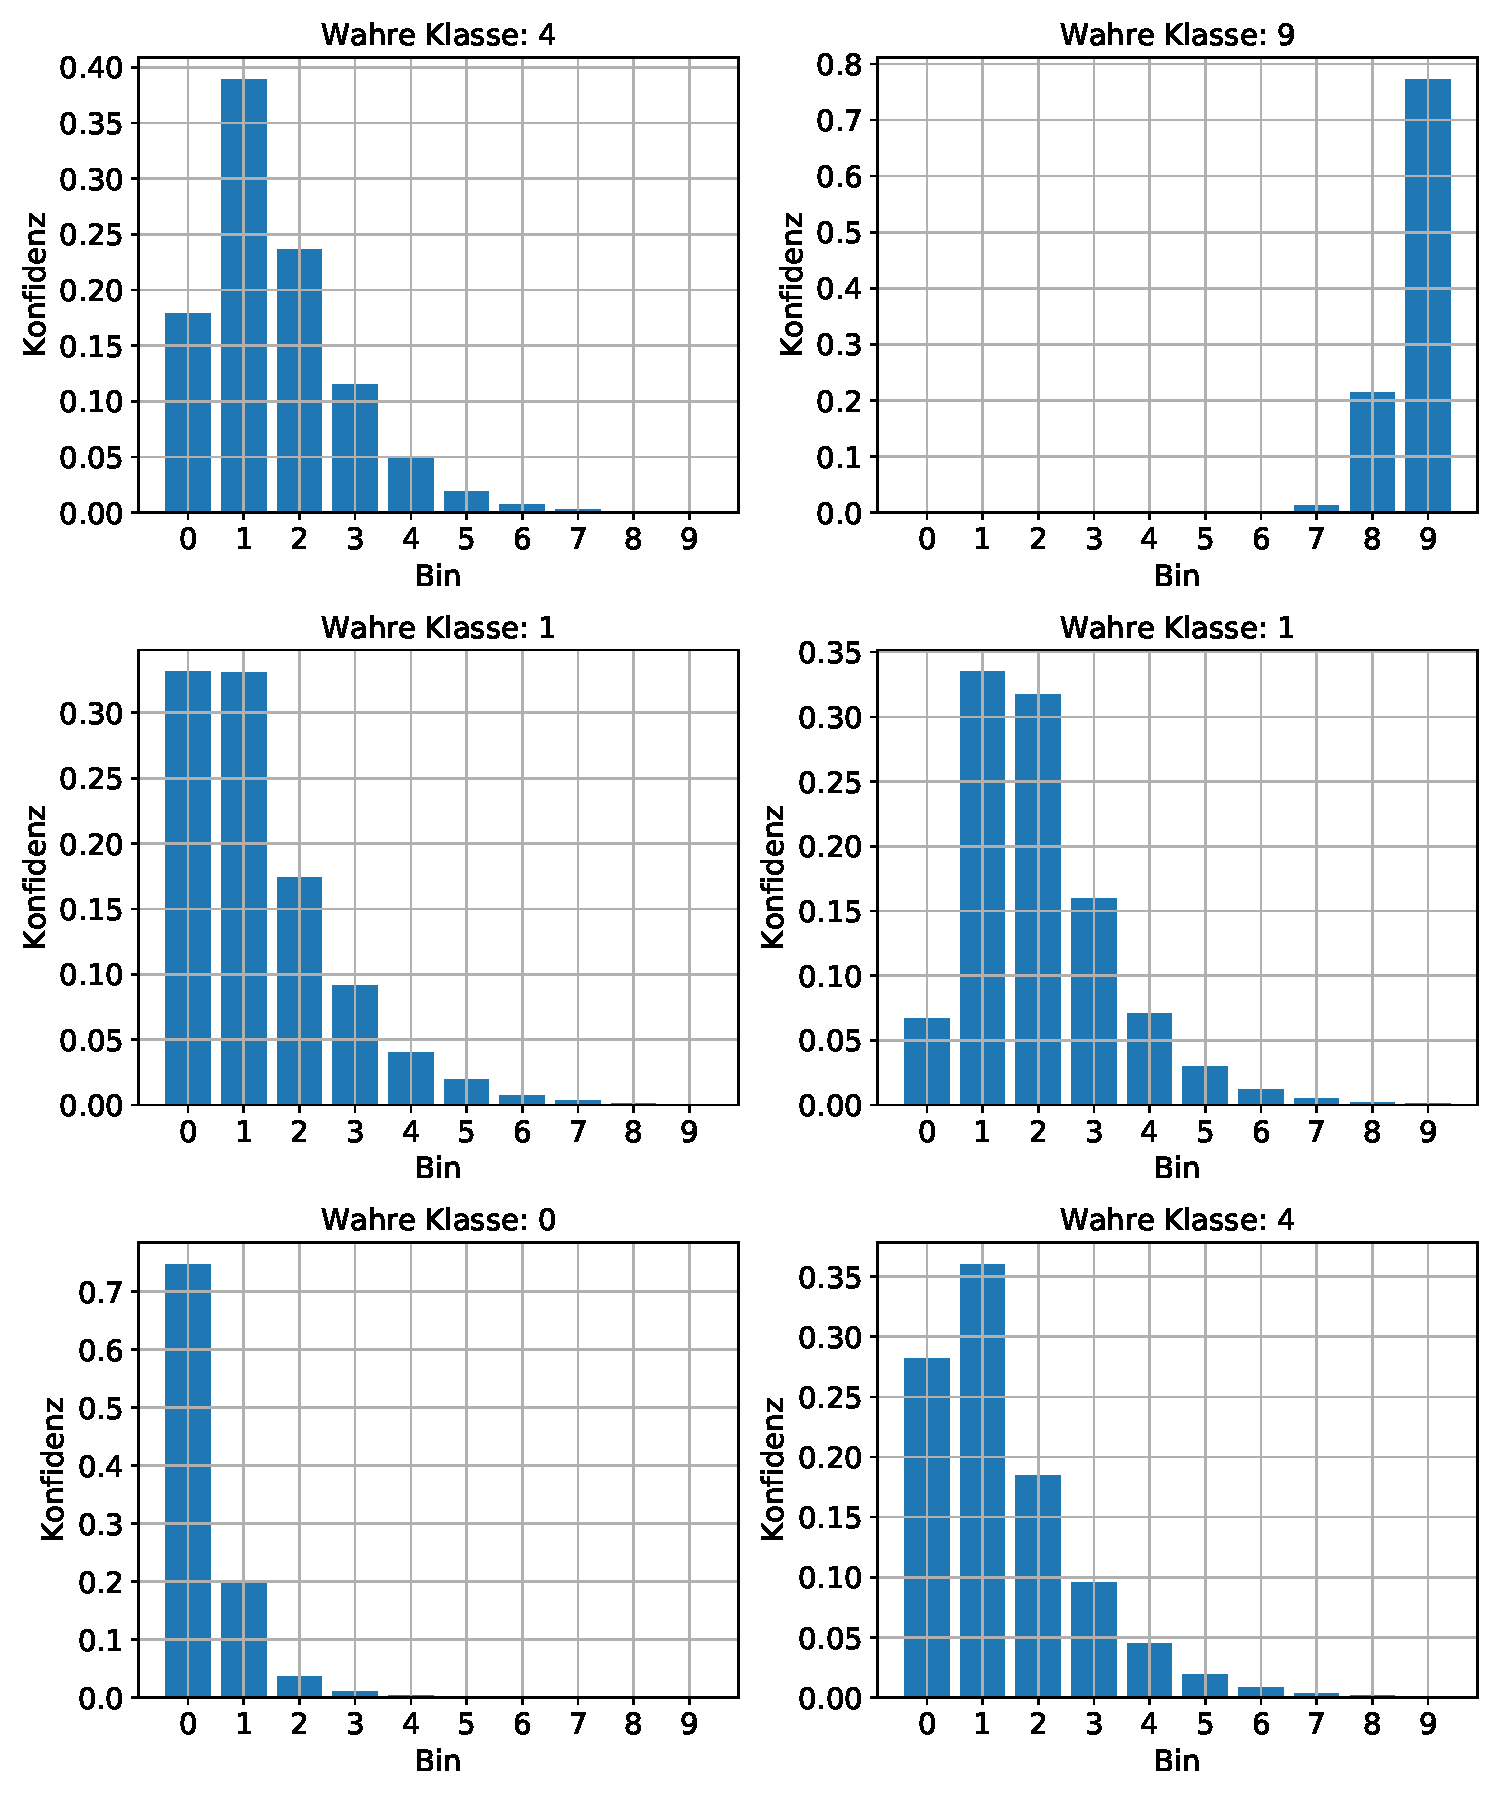
\includegraphics[width=\textwidth]{Plots/NN/single_events.pdf}%
    \caption[Vorhersage einzelner Events des NN ohne DSEA]{Vorhersage einzelner Events des NN.
    Jedem Energie-Bin wird eine Konfidenz zugeordnet.
    Diese gibt die Wahrscheinlichkeit an, dass das betrachtete Event zu dem Energie-Bin gehört.
    }%
    \label{fig:NN_single_events}%
\end{figure}%

